\begin{figure}
\centering
\begin{tikzpicture}[declare function={f(\x,\y)=20-(\x)^4-(\y)^2;}]
\pgfmathsetmacro{\kxs}{1.2}
\pgfmathsetmacro{\kxe}{\kxs+0.3}
\pgfmathsetmacro{\kxm}{\kxs+0.2)}
\pgfmathsetmacro{\kys}{-0.3}
\pgfmathsetmacro{\kye}{0.3}
  \begin{axis}[clip=false,axis on top,view/h=160,small,axis lines=center,colormap={kgray}{gray(0.2cm)=(0.6);gray(1cm)=(0.9);},xtick={\empty},ytick={\empty},ztick={\empty},enlargelimits=true,
%xmax=2,ymax=1.5,zmax=0.5,
,xlabel={},ylabel={},zlabel={},xlabel style={anchor=east},ylabel style={anchor=west},zlabel style={anchor=east},
axis line style={draw=none}]
\addplot3[surf,faceted color=white,domain=0.5:1.8,domain y=-1:1]({x},{y},0);
\addplot3[surf,,faceted color=black,,domain=\kxs:\kxe,domain y=\kys:\kye]({x},{y},0);
%\addplot3[dashed]coordinates {(\kxs-\kya,0)(\kxs-\kya,{f(\kxs-\kya)})};
%\addplot3[dashed]coordinates {(\kxe-\kya,0)(\kxe-\kya,{f(\kxe-\kya)})};
%\addplot3[dashed]coordinates {(\kxe\kya,0)(\kxe\kya,{f(\kxe\kya)})};
%\addplot3[dashed]coordinates {(\kxs\kya,0)(\kxs\kya,{f(\kxs\kya)})};
\addplot3[surf,shader=flat, faceted color=none,domain=0.5:1.8,domain y=-1:1]{f(x,y)};
\addplot3[]coordinates{(1.5,-1.5,{f(1.5,-1.5)})}node[above left]{$S$};
\addplot3[]coordinates{(1.5,0,0)}node[below left]{$R$};
\addplot3[surf,faceted color=gray,domain=\kxs:\kxe,domain y=\kys:\kye]{f(x,y)};
%\addplot3[surf, faceted color=lgray,domain=\kxs:\kxe,domain y=-\kya:\kya](x,y,{f(\kxs,-0.3)});
\addplot3[fill=lgray]coordinates {(\kxs,\kys,{f(\kxs,\kys)}) (\kxe,\kys,{f(\kxm,\kys)}) (\kxe,\kye,{f(\kxm,\kye)}) (\kxs,\kye,{f(\kxs,\kye)}) (\kxs,\kys,{f(\kxs,\kys)}) };
%\addplot3[]coordinates {({\kxs},{\kya},0)}node[right]{$\Delta A_k$};
%\addplot3[]coordinates {({\kxs+0.1},{\kya+0.1},{f(\kxs\kya)})}node[pin=20:{$\Delta \sigma_k$}]{};
%\addplot3[]coordinates {({\kxs},{-\kya},{f(0,0)})}node[pin=30:{$\Delta P_k$}]{};
\end{axis}
\end{tikzpicture}
\end{figure}


\begin{figure}
\centering
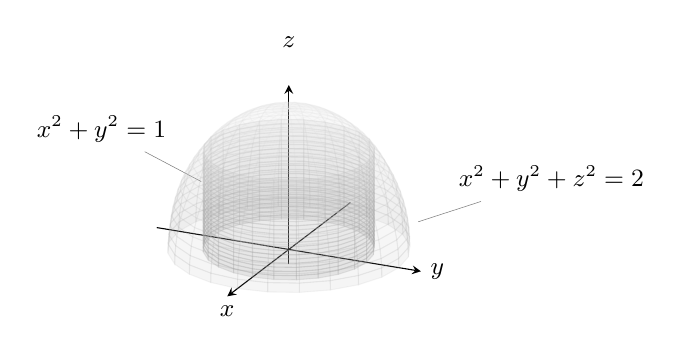
\begin{tikzpicture}[font=\small,declare function={fx(\t,\p)=sqrt(2)*cos(\t)*sin(\p);fy(\t,\p)=sqrt(2)*sin(\t)*sin(\p);fz(\t,\p)=sqrt(2)*cos(\p);
gx(\t,\z)=1*cos(\t);gy(\t,\z)=1*sin(\t);gz(\t,\z)=\z;}]
\begin{axis}[view/h=115,clip=false,axis lines=center,small,colormap={}{gray(0cm)=(0.6);gray(1cm)=(0.9);},enlargelimits=true,xlabel={$x$},ylabel={$y$},zlabel={$z$},xlabel style={anchor=north},ylabel style={anchor=west},zlabel style={anchor=south,yshift=1em},xtick={\empty},ytick={\empty},ztick={\empty},zmax=1.5,]
\addplot3[]coordinates {({gx(-90,0.5)},{gy(-90,0.5)},{gz(-90,0.5)})}node[pin=135:{$x^2+y^2=1$}]{};
\addplot3[surf,opacity=0.2,faceted color=none,z buffer=sort,domain=0:360,domain y=0:1]({gx(x,y)},{gy(x,y)},{gz(x,y)});
\addplot3[surf,opacity=0.1,faceted color=none,z buffer=sort,domain=0:360,domain y=0:90]({fx(x,y)},{fy(x,y)},{fz(x,y)});
\addplot3[]coordinates {({fx(115,80)},{fy(115,80)},{fz(115,80)})}node[pin=30:{$x^2+y^2+z^2=2$}]{};
\end{axis}
\end{tikzpicture}
\end{figure}

\begin{figure}
\centering
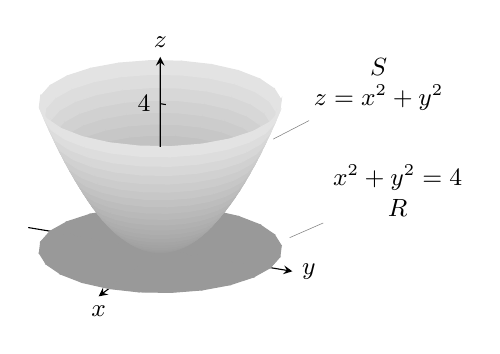
\begin{tikzpicture}[font=\small,declare function={fx(\r,\t)=\r*cos(\t);fy(\r,\t)=\r*sin(\t);fz(\r,\t)=\r^2;}]
\begin{axis}[view/h=115,clip=false,axis lines=center,small,colormap={}{gray(0cm)=(0.6);gray(1cm)=(0.9);},enlargelimits=true,xlabel={$x$},ylabel={$y$},zlabel={$z$},xlabel style={anchor=north},ylabel style={anchor=west},zlabel style={anchor=south,yshift=1em},xtick={\empty},ytick={\empty},ztick={\empty},zmax=4.1,
%hide axis
]
\addplot3[surf,faceted color=none,z buffer=sort,domain=0:2,domain y=0:360]({fx(x,y)},{fy(x,y)},{0});
\addplot3[surf,faceted color=none,z buffer=sort,domain=0:2,domain y=0:360]({fx(x,y)},{fy(x,y)},{fz(x,y)});
\addplot3[-stealth]coordinates {({fx(2,25)},{fy(2,25)},{fz(2,25)}) ({fx(2,205)},{fy(2,205)},{fz(2,205)+0.1})};
\addplot3[]coordinates {({0},{0},{fz(2,25)}) ({0},{0.1},{fz(2,25)})}node[pos=0,left]{$4$};
\addplot3[]coordinates {({fx(1.7,115)},{fy(1.7,115)},{fz(1.7,115)})}node[pin={[align=center]30:{$S$\\$z=x^2+y^2$}}]{};
\addplot3[]coordinates {({fx(2,125)},{fy(2,125)},{0})}node[pin={[align=center]20:{$x^2+y^2=4$\\$R$}}]{};
\end{axis}
\end{tikzpicture}
\end{figure}



\begin{figure}
\centering
\begin{tikzpicture}[font=\small,declare function={fx(\x,\y)=\x;fy(\x,\y)=\x^2;fz(\x,\y)=1-\x^2;}]
\pgfmathsetmacro{\kx}{0.35}
\pgfmathsetmacro{\ky}{\kx^2}
\pgfmathsetmacro{\kz}{1-\ky}
\begin{axis}[clip=false,view/h=145,small,axis lines=middle,xtick={1},ytick={1},ztick={1},enlargelimits=true, xlabel={$x$}, ylabel={$y$},zlabel={$z$}, xlabel style={anchor=north},ylabel style={anchor=west},zlabel style={anchor=south},colormap={}{gray(0cm)=(0.6);gray(1cm)=(0.9);},xmax=1.25,ymax=1.25,zmax=1.25]
\addplot3[black,domain=-1:1,domain y=0:1]({fx(x,y)},{fy(x,y)},{fz(x,y)});
\addplot3[domain=-1:1,samples y=0]({x},{x^2},{0})node[pos=0,right]{$(-1,1,0)$}node[pos=1,below]{$(1,1,0)$};
\addplot3[]coordinates{(\kx,\ky,0)(\kx,\ky,\kz)}node[pos=0.5,pin={[align=center]135:{\text{\RL{اطراف}}\\$y=x^2$}}]{};
\addplot3[]coordinates{(-0.4,0.5,0.5)}node[pos=0.8,pin={[align=center]45:{\text{\RL{بالائی سطح}}\\$y+z=1$}}]{};
\end{axis}
\end{tikzpicture}
\end{figure}


\begin{figure}
\centering
\begin{tikzpicture}[declare function={f(\x,\y)=16-\x^2-2*(\y-1)^2;g(\x,\y)=14+6*\y;}]
\pgfmathsetmacro{\kxaa}{1.0}
\pgfmathsetmacro{\kxa}{1.5}
\pgfmathsetmacro{\kya}{1.3}
  \begin{axis}[clip=false,axis on top,view/h=100,small,axis lines=center,colormap={kgray}{gray(0.2cm)=(0.6);gray(1cm)=(0.9);},xtick={\empty},ytick={\empty},ztick={\empty},enlargelimits=true,
%xmax=2,ymax=1.5,zmax=0.5,
,xlabel={},ylabel={},zlabel={},xlabel style={anchor=east},ylabel style={anchor=west},zlabel style={anchor=east},
axis line style={draw=none}
]
\addplot3[surf,faceted color=none,domain=0:-1.5,domain y=0:1.1](x,y,0);
\addplot3[surf,faceted color=none,domain=0:-1.5,domain y=0:1.1]{f(x,y)};
\addplot3[surf,,faceted color=none,domain=0:-1.5,domain y=0:1.1]{g(x,y)};
%
\addplot3[-latex] coordinates {(0,0,{f(0,0)}) (0,0,{f(0,0)+10})}node[pos=1,above]{$\kvec{p}$}coordinate[pos=0.6] (kA);
\addplot3[-latex] coordinates {(0,0,{f(0,0)}) (0,-0.2,{f(0,0)+9})}node[pos=1,left]{$\nabla f(x_k,y_k)$}coordinate[pos=0.5] (kB);
\addplot3[-latex] coordinates {(0,0,{f(0,0)}) (0,1.1,{g(0,1.1)})}node[pos=0.8,above]{$\kvec{u}_k$};
\addplot3[-latex] coordinates {(0,0,{f(0,0)}) (-1.5,0,{g(1.5,0)})}node[pos=1,above]{$\kvec{v}_k$};
\addplot3[] coordinates {(0,0,{f(0,0)})}node[circ]{}node[pin=190:{$T_k$}]{};
\addplot3[] coordinates {(0,0,0)}node[circ]{}node[left]{$c_k$};
\addplot3[]coordinates {(-1.5,1.1,{f(x,y)})}node[right]{$\Delta \sigma_k$};
\addplot3[]coordinates {(-1.5,1.1,{g(x,y)})}node[above]{$\Delta P_k$};
\addplot3[]coordinates {(-1.5,1.1,0)}node[right]{$\Delta A_k$};
\addplot3[-latex]coordinates {(0,0,0) (0,0,8)}node[pos=0.75,left]{$\kvec{p}$};
\end{axis}
\draw(kB) to [out=45,in=135] node[pos=0.4,above,xshift=-0.20em]{\footnotesize $\gamma_k$}(kA);
\end{tikzpicture}
\end{figure}


\begin{figure}
\centering
\begin{tikzpicture}[declare function={f(\x,\y)=16-\x^2-2*(\y-1)^2;g(\x,\y)=14+6*\y;}]
\pgfmathsetmacro{\kxaa}{1.0}
\pgfmathsetmacro{\kxa}{1.5}
\pgfmathsetmacro{\kya}{1.3}
  \begin{axis}[clip=false,axis on top,view/h=100,small,axis lines=center,colormap={kgray}{gray(0.2cm)=(0.6);gray(1cm)=(0.9);},xtick={\empty},ytick={\empty},ztick={\empty},enlargelimits=true,
%xmax=2,ymax=1.5,zmax=0.5,
,xlabel={},ylabel={},zlabel={},xlabel style={anchor=east},ylabel style={anchor=west},zlabel style={anchor=east},
axis line style={draw=none}
]
\addplot3[black,domain=0:1,samples y=0](x,0,{f(x,0)}) ;
\addplot3[black,domain=0:1,samples y=0](x,1,{f(x,1)});
\addplot3[black,domain=0:1,samples y=0](0,x,{f(0,x)});
\addplot3[black,domain=0:1,samples y=0](1,x,{f(1,x)});
%\addplot3[surf,,faceted color=none,domain=0:-1.5,domain y=0:1.1]{g(x,y)};
\end{axis}
\end{tikzpicture}
\end{figure}

